\documentclass[11pt,a4paper,oneside,parskip=half,DIV=8,BCOR=10mm]{scrbook}

\usepackage[sc]{mathpazo} % Use the Palatino font
\usepackage[T1]{fontenc} % Use 8-bit encoding that has 256 glyphs
\linespread{1.0} % Line spacing - Palatino needs more space between lines
\usepackage{microtype} % Slightly tweak font spacing for aesthetics

\usepackage[hmarginratio=1:1,top=32mm,columnsep=20pt]{geometry} % Document margins
\usepackage{multicol} % Used for the two-column layout of the document
\usepackage{multirow}
\usepackage{longtable}
\usepackage[hang, small,labelfont=bf,up,textfont=it,up]{caption} % Custom captions under/above floats in tables or figures
\usepackage{booktabs} % Horizontal rules in tables?
\usepackage{float} % Required for tables and figures in the multi-column environment - they need to be placed in specific locations with the [H] (e.g. \begin{table}[H])

\makeatletter
\let\@tmp\@xfloat
\usepackage{fixltx2e}
\let\@xfloat\@tmp
\makeatother

\usepackage{hyperref} % For hyperlinks in the PDF
\usepackage{lettrine} % The lettrine is the first enlarged letter at the beginning of the text
\usepackage{paralist} % Used for the compactitem environment which makes bullet points with less space between them
\usepackage{listings}
\usepackage{amsmath}
\usepackage{empheq}
\usepackage{amsfonts}
\usepackage{amssymb}
\usepackage[usenames,dvipsnames]{xcolor} %color changes
\usepackage{graphicx}
\usepackage{subfigure}
\usepackage[normalem]{ulem}
\usepackage{stmaryrd}
\usepackage{csquotes}
\usepackage{caption}
%\usepackage{subcaption}
\usepackage{fancyvrb}
\usepackage{pdfpages}
\usepackage{rotating}
\usepackage{siunitx}
\sisetup{math-micro=\text{µ},text-micro=µ}
\usepackage{glossaries}
\usepackage{gensymb}
\usepackage{wrapfig}

\usepackage[usenames,dvipsnames]{xcolor}
\usepackage{fontspec}
\definecolor{bgcolor}{rgb}{1, 1, 1}
\definecolor{codecolor}{rgb}{0, 0, 0}
\definecolor{stringcolor}{rgb}{0.62, 0, 0.36}
\definecolor{keywordcolor}{rgb}{0, 0, 0}
\definecolor{commentcolor}{rgb}{0.66, 0.66, 0.61}
\definecolor{linenumbercolor}{rgb}{0.4, 0.4, 0.4}
\definecolor{directivecolor}{rgb}{0, 0, 0}
\newfontfamily\listingsfont[Scale=.8]{Roboto}

\lstdefinelanguage{CustomAndroid}[]{C++} {
	morekeywords    = {*, func, var, let, nil, guard, protocol, extension, import, in, inout, typealias, associatedtype, precedencegroup},
	directivestyle  = \listingsfont\bfseries\color{directivecolor},
	morecomment=[n]{/*}{*/},    % allows for nested multi-line comments
}

\lstdefinestyle{Basic}{
	xleftmargin=15pt,
	backgroundcolor         = \color{bgcolor},
	fillcolor               = \color{bgcolor},
	basicstyle              = \linespread{1.0}\color{codecolor}\scriptsize\listingsfont,
	commentstyle            = \color{commentcolor},                  
	keywordstyle            = \listingsfont\bfseries\color{keywordcolor},
	identifierstyle         = ,
	numberstyle             = \color{linenumbercolor},                        % the style that is used for the line-numbers
	stringstyle             = \color{stringcolor},                            % string literal style
	breakatwhitespace       = false,                                          % sets if automatic breaks should only happen at whitespace
	breaklines              = true,                                           % sets automatic line breaking
	escapeinside            = {\%*}{*)},                                      % if you want to add LaTeX within your code
	extendedchars           = true,                                           % lets you use non-ASCII characters; for 8-bits encodings only
	rulesep                 = 5pt,
	framexleftmargin        = 2pt,
	framerule               = 0.5pt,
	framesep                = 1pt,
	keepspaces              = true,                                           % keeps spaces in text, useful for keeping indentation of code
	morekeywords            = {*,interface},      	 	  % if you want to add more keywords to the set
	numbers                 = left,                               % where to put the line-numbers; possible values are (none, left, right)
	numbersep               = 6pt,                                % how far the line-numbers are from the code
	showspaces              = false,                              % show spaces everywhere adding particular underscores
	showstringspaces        = false,                              % underline spaces within strings only
	showtabs                = false,                              % show tabs within strings adding particular underscores
	stepnumber              = 1,                                  % the step between two line-numbers. If it's 1, each line will be numbered
	tabsize                 = 2,                                  % sets default tabsize to 2 spaces
	title                   = \lstname,                           % show the filename of files included with \lstinputlisting
}



\usepackage[backend=biber,style=alphabetic]{biblatex}
\addbibresource{database.bib}

\title{GPU Databases}
\subtitle{}
\subject{Seminar}
\author{Samuel Kurath}
\date{MSE Database Seminar - Fall 2017}
\publishers{Supervised by Prof. Stefan Keller}


\hypersetup{
	pdfauthor={Samuel Kurath},
	pdftitle={GPU Databases},
	hidelinks
}

\newglossaryentry{Azimuth}{
    name={Azimuth},
    description={Degrees of rotation about the z axis. The angle between the device's current compass direction and magnetic north}
}

\newglossaryentry{Pitch}{
    name={Pitch},
    description={Degrees of rotation about the x axis. The angle between a plane parallel to the device's screen and a plane parallel to the ground}
}

\newglossaryentry{Roll}{
    name={Roll},
    description={Degrees of rotation about the y axis. The angle between a plane perpendicular to the device's screen and a plane perpendicular to the ground}
}


\newglossaryentry{GeoJSON}{
    name={GeoJSON},
    description={GeoJSON is an open standard format designed for representing simple geographical features}
}

\newglossaryentry{covariance}{
    name={covariance},
    description={Covariance provides a measure of the strength of the correlation between two or more sets of random variables}
}





\makeglossaries

\begin{document}

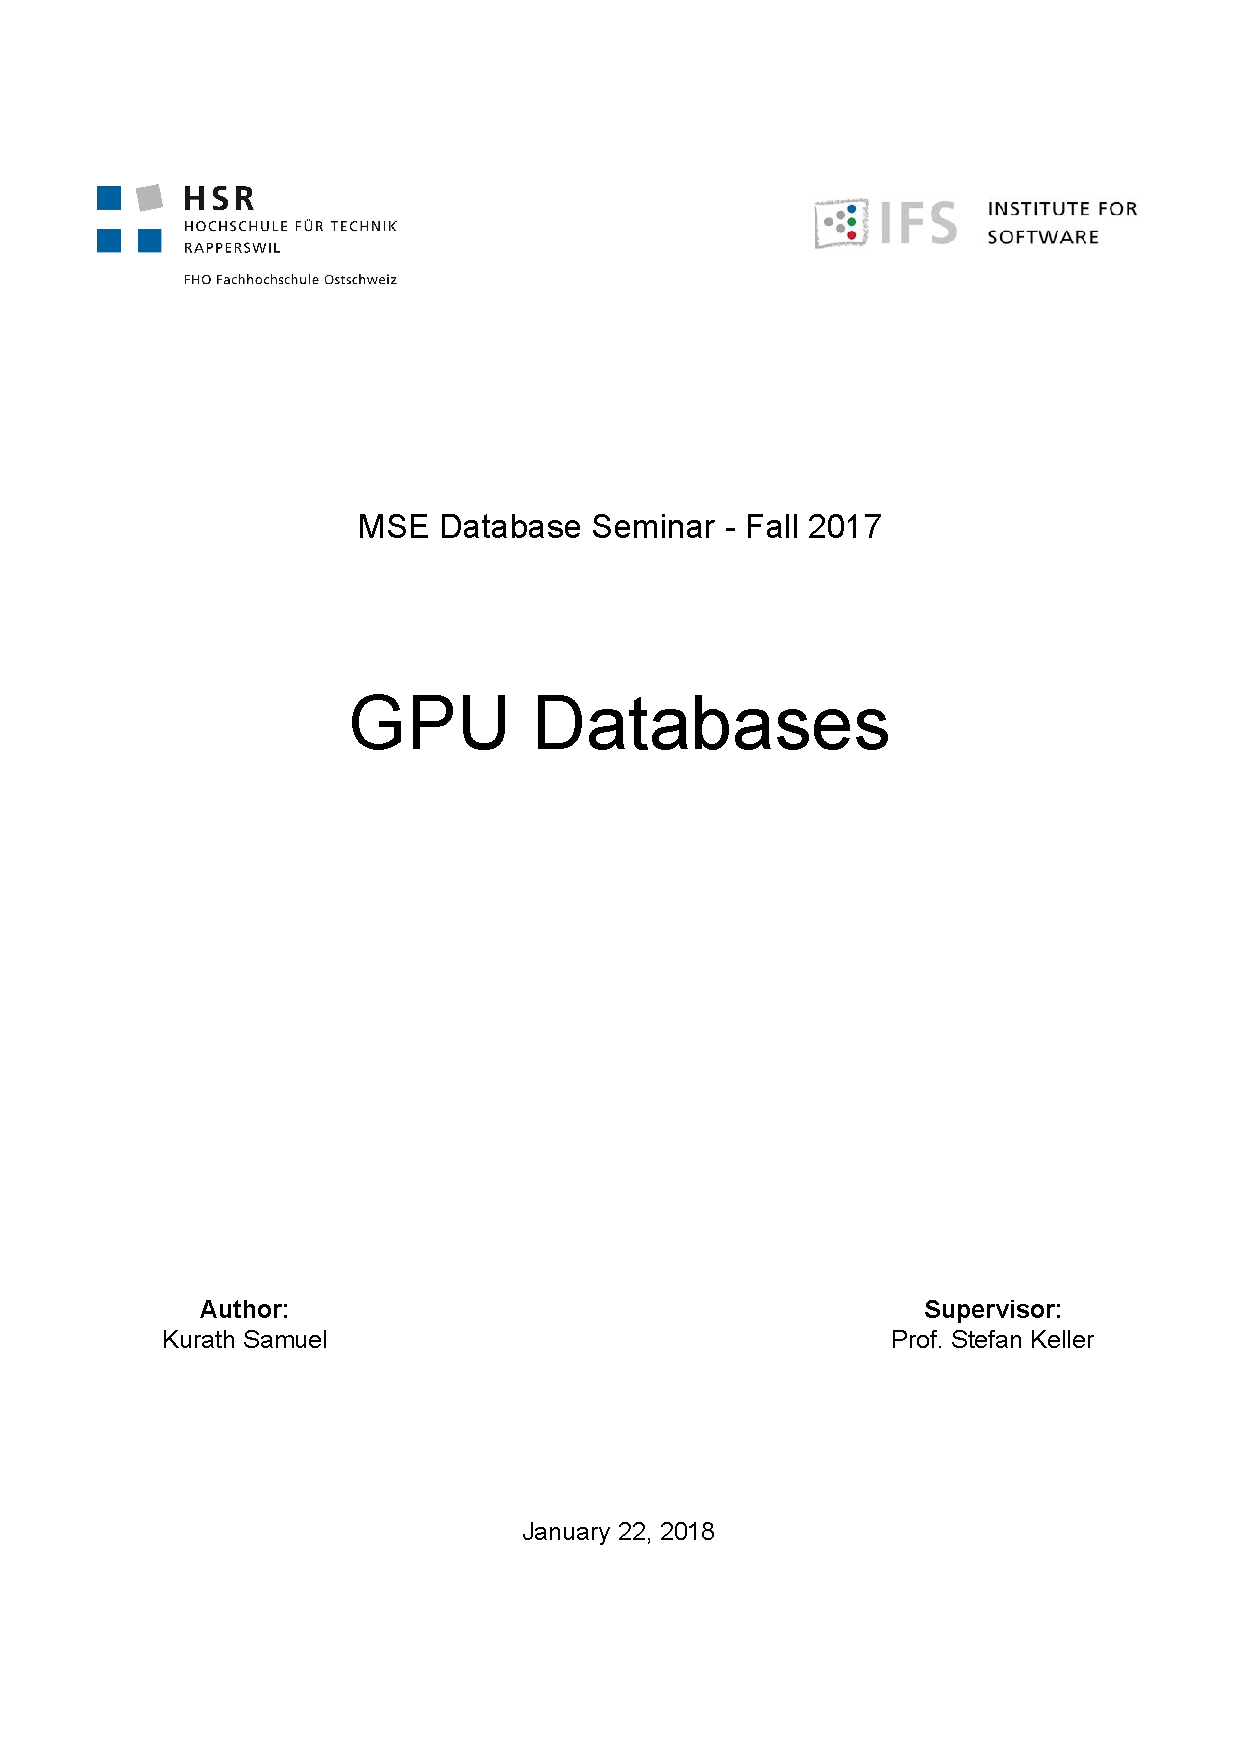
\includepdf[pages={1}]{pdfs/Gpu_Seminar_Titel.pdf}
\cleardoublepage

%\let\oldsection\section
%\renewcommand\section{\clearpage\oldsection}

\pagestyle{headings}
\setcounter{page}{1}
\pagenumbering{Roman}

\chapter*{Abstract}
The content of this paper is splitted into three parts, it begins with an overview about GPU Database Systems.
Followed by a port about MapD, that is an example of the available GPU database products.
And finally a benchmark comparing the performance of MapD and PostgreSQL.
The data of the benchmark is based on a part of the Unified New York City Taxi and Uber data.
\cleardoublepage

\setcounter{page}{1}
\pagenumbering{arabic}

\tableofcontents

\chapter{Introduction}
\label{introduction}

Durring the Master of Science in Engineering the students have to participate at two seminars.
The goal of these are to elaborate a theme on their own, discuss the result in group and write a paper about the topic.

The Databasesystems Seminar does a focus on GPU Database Systems.
The students do have a closer look at a certain GPU Database product and have to do a benchmark.

The benchmark is based on the public NYC Taxi Rides dataset and the queries are predetermined by Prof. Stefan Keller.


\chapter{GPU Databases}
Related to the massive amount of data that is collected nowadays, the stagnation of CPU speed
and the trend to use the GPU for tasks like machine learning, the database developers have discovered the GPU to improve the performance of their products, too.
Hence the main idea of GPU databases is to perform some operations on the GPU for acceleration purposes.

\paragraph{Strengths}
GPUs do have their strengths on parallelable tasks.
This is due to the fact that GPUs can have thousands of cores and high bandwidth memory on each card.
Thus most of the GPU databases products focus on analytics.


\paragraph{Weaknesses} Beside of these strengths, GPU databases host several pitfalls like transfer of the data from the CPU to the GPU,
 the memory limitations and the massiv costs of GPU servers.


\section{Components of a GPU database}
The current section will give you an overview of the components a GPU database consists of.
The paper \cite{bress2014gpu} of Sebastian Bress et al. does split the components into Functional and Non-Functional properties.
Since those categories are reasonable they are used in this paper as well.
The next sub section will explain and list these properties.

\subsection{Non-Functional properties}

\subsubsection{Performance}
Performance is the biggest advantage of GPU database, but not all tasks are automatic faster on GPUs.
Due to the huge amount of processors tasks that are able to parallelise easily are incredibly fast.
Unfortunately task which require a complex control flow or are hard to parallelise don't profit from the cores.
And there is always the bottleneck of the data transfer to the GPU.

\subsubsection{Portability}
In terms of portability we talk about if the GPU database is able to run on different GPUs or CPUs vendors/architectures, like NVIDIA or AMD graphic cards.
Often this requirement is in contrast to the performance property, since the vendors offer special implementation or hardware details to accelerate their products.

\subsubsection{Scalability}
To my point of view the paper \cite{bress2014gpu} of Sebastian Bress et al. missed the important criteria of the scalability.
The collected data of companies grow and grow, thus you need to have memory for all that data. Sadly the memory of GPUs is often limited,
hence the only way to handle this issue it to scale your GPU database verticaly over multiple GPUs.

\subsection{Functional properties}

\subsubsection{Storage system}
If we talk about storage systems there are several scenarios conceivable.
First with the Video Random Access Memory (VRAM) of the GPUs we have an additional storage medium next to the Random-Access Memory (RAM) and the hard disk.
The different mediums provide different advantages and disadvantages.
Hard disks are persistent, cheap and have a huge capacity.
Unfortunately they are pretty slow.
Random-Access Memory is very fast compared to hard disks but the transfer to the GPU is still a bottleneck and it isn't a persistent storage, either.
With Video Random Access Memory the bottleneck of the transfer disappears, but most of the time the storage capacity is highly limited.

\subsubsection{Storage model}
In terms of storage model, there are row stores or column stores \cite{abadi2008column}.
Row stores store table records in a sequence of rows.
Column stores store table records in a sequence of columns, the entries of a column is stored in contiguous memory locations \cite{bress2014design}.
The advantages of column stores are tasks like aggregations, though row stores are more efficient if the result of a query returns multiple rows.


\subsubsection{Processing model}
There are two processing models in modern databases tuple-at-a-time and operator-at-a-time.
The tuple-at-a-time is similar to an iterator, which iterates over the relevant tuples and applies the operations.
The operator-at-a-time fits to GPUs, since it applies the same operation on a bulk of data.

\subsubsection{Query processing}
GPU database systems are able to use the GPU and the CPU, hence it is necessary to choose the right processor for the right task.
\paragraph{Query placement} It is a extremely difficult task to decide which processing device is the most accurate for the current query.
\paragraph{Optimization} To optimize the performance in therms of query execution time, several factors are include.
For example the operations, the data, hardware specifications and even more.

\subsubsection{Transaction support}
An other problem are transactions and consistency on GPUs, until now there is almost no research done in this area.
Thus most of the GPU database don't support transactions.


\subsection{Proposed architecture}
The paper \cite{bress2014gpu} proposes an architecture with an in-memory storage, using a column store, an operator-at-a-time processing model, cross device processing and no transaction support.
With regard to the portability a hardware oblivious architecture is suggested.
To my point of view a hardware aware GPU database would make more sense.
Since GPU databases are all about speed, use hardware specific tuning would result in more acceleration.
And the huge amount of data makes scalability absolutely necessary.

\chapter{MapD}

\begin{wrapfigure}{r}{0.2\textwidth}
  \begin{center}
    
\includegraphics[width=100pt]{images/mapd_logo.png}
  \end{center}
  \caption[MapD]{MapD Logo}
\end{wrapfigure}


MapD is a GPU database with the goal to speed up queries and analytic tasks with the power of GPU's
and their massive parallel architectures consisting of thousands of cores.
The first prototype of MapD was develop in 2012 by Todd Mostak.
A year leater MapD was incubated at the  MIT’s Computer Science and Artificial Intelligence Laboratory (CSAIL) database group
and in September 2013 Todd Mostak founded MapD Technologies, Inc.
They have got two products called MapD Core \cite{mapdcore} and MapD Immerse \cite{immerse}.
The MapD Core SQL engine is an open source in-memory, SQL, GPU database and
MapD Immerse is a tool for visual analytics on top of MapD Core SQL engine.


\begin{figure}[H]
    \centering
    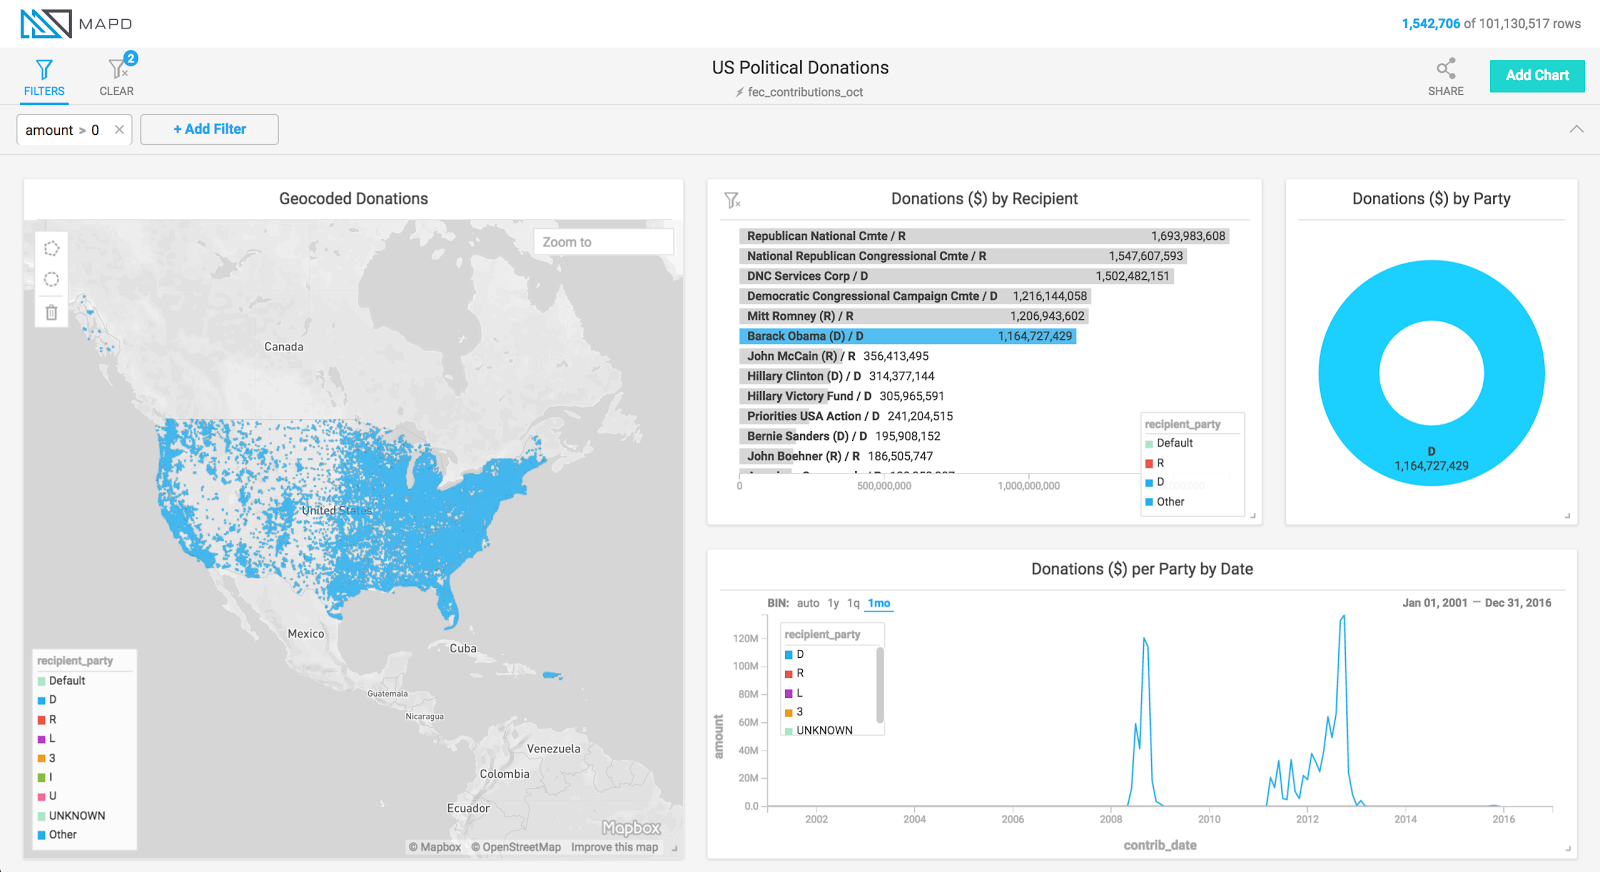
\includegraphics[width=0.9\textwidth,height=0.9\textheight,keepaspectratio]{images/mapd_imerse.png}
    \caption{MapD Immerse \cite{filtering}}
    \label{fig:immerse}
\end{figure}


\newpage
\subsection{Functional Properties}
Related to the excellent Survey of Sebastian Bress et al. \cite{bress2014gpu} MapD has the following functional properties.

\paragraph{Storage system} MapD has got a relational DBMS that is able to handle data amounts bigger than the memory space.
But tries to hold as much data as possible in-memory to to improve the performance.
\paragraph{Storage model} MapD uses a columnar layout to store the data and uses so called chunks, which split the columns in smaller pieces.
The chunks are the basic units of the memory manager.
\paragraph{Processing model} MapD processes on operator-at-a-time or one chunk per operation. Thus it is a block-oriented processing.
The queries are compiled for the CPU and the GPU.
\paragraph{Query placement} In contrast to \cite{bress2014gpu} the gained experience with MapD showed that MapD tries to run the queries on the GPU even if there isn't enough space and isn't able to handle such queries on his own.
°Hence the user had to switch the execution mode from GPU to CPU.
\paragraph{Optimization} MapD's optimizer tries to execute the queries on the most suitable device, like text searching using an index on the CPU and table scans on the GPU.
\paragraph{Transactions} MapD does not support transactions.


\newpage
\section{Overview}

The following section will give you an overview about the handling of MapD.
Often there will be a comparison between MapD and PostgreSQL to point out the differences and similarities of these two databases.



\subsection{Data Definition Language (DDL)}
The DDL seams familiar since it uses SQL syntax \cite{ddl}.
The syntax to handle users, databases, tables, and views is as listed below.

\paragraph{User}
\begin{itemize}
 \item CREATE USER
 \item DROP USER
 \item ALTER USER
\end{itemize}

\paragraph{Database}
\begin{itemize}
 \item CREATE DATABASE
 \item DROP DATABASE
\end{itemize}


\paragraph{Table}
\begin{itemize}
 \item CREATE TABLE
 \item CREATE TABLE AS SELECT
 \item ALTER TABLE
 \item DROP TABLE
 \item TRUNCATE TABLE
\end{itemize}

\paragraph{View}
\begin{itemize}
 \item CREATE VIEW
 \item DROP VIEW
\end{itemize}


\subsubsection{Datatypes}
MapD supports the data types shown in table \ref{tab:datatypes}.
To get a better intuition the corresponding PostgreSQL data types are listed as well.

\begin{table}[H]
\centering
\begin{tabular}{ |l|l|l|l| }
\hline
\multicolumn{2}{| l |}{MapD} & \multicolumn{2}{| l |}{PostgreSQL}  \\
\hline
Data type & Size [bytes] & Data type & Size [bytes]  \\
\hline
TEXT & Variable & text & Variable \\
TIMESTAMP	& 8 & timestamp & 8 \\
TIME	& 8 & time & 8 \\
DATE	& 8 & date &  4 \\
FLOAT	& 4 & real & 4 \\
DOUBLE	& 8 & double precision & 8 \\
INTEGER	& 4 & integer & 4 \\
SMALLINT & 2 & smallint & 2 \\
BIGINT	& 8 & bigint & 8 \\
BOOLEAN	& 1 & boolean & 1 \\
DECIMAL	& 8 & numeric & variable \\
\hline
\end{tabular}
\caption{Data types \cite{mapddatatype} \cite{postgresdatatype}}
\label{tab:datatypes}
\end{table}

As you can see MapD supports the common data types.
And if you compare them to the corresponding PostgreSQL types they have got nearly the same names.
In addition PostgreSQL provides further data types like json or box which allow extended possibilities of use.


\subsection{Data Manipulation Language (DML)}
As well as the DDL of MapD the DML uses the SQL syntax too.
MapD currently supports the instructions:
\begin{itemize}
 \item INSERT INTO
 \item SELECT
\end{itemize}

Until now there is no support for the operations:
\begin{itemize}
 \item DELETE
 \item UPDATE
\end{itemize}
But they are in development, since MapD don't want to compromising the speed much with these instructions it may take a while.

Furthermore, MapD provides operations like EXPLAIN, LIKELY/UNLIKELY, Aggregate Functions and Conditional Expressions to improve the DML operations and extend the functionality.

\subsection{Data import}
MapD allows to import data from different sources as you can see in the following section.

\subsubsection{COPY FROM}
The COPY FROM operation is callable from the mapdql terminal and imports data from a local CSV or related format file into the database.

\subsubsection{SQL Importer}
The SQL Importer is a java tool that allows to run queries on other database via JDBC and stores the results in to MapD.

\subsubsection{StreamInsert}
The StreamInsert program could be attached at the end of a real-time stream processing engine like Kafka or a similar product to import stream data into MapD for further analytic tasks.

\subsubsection{HDFS}
The tool sqoop-export offers the possibility to import CSV or Parquet files from a HDFS file system into MapD database.

\subsection{Data export}
To export data from MapD, mapdql provides the command COPY TO that allows to export the result of a SELECT statement to a file.
For example like:
\begin{itemize}
 \item COPY (SELECT * FROM tweets) TO '/tmp/tweets.csv';
\end{itemize}


\newpage
\subsection{Client interfaces}
MapD provides a tool called mapdql \cite{mapdql} as a client-side SQL console that displays query results you submit to the MapD Core Server.
The counterpart of PostgreSQL is psql \cite{psql}.

\subsubsection{Database connection}
To following commands compares the connection to MapD respectively PostgreSQL with mapdql and psql.
\begin{itemize}[noitemsep]
 \item[mapdql:]  mapdql <database>  -u <user> -p <password> --port <port> -s <host>
 \item[pgsql:]  psql -h <host> -p <port> -U <user> -W <password> <database>
\end{itemize}

\subsubsection{Commands}
The table \ref{tab:commands} lists some basic commands of mapdql and pgsql.
It is only a slight slice of all possible commands, but another good example to point out how much in common those two products have.
\begin{table}[H]
\centering
\begin{tabular}{ |l|l|l| }
\hline
Command & mapdql & pgsql  \\
\hline
	List databases & \textbackslash l &  \textbackslash l \\
	List tables in database & \textbackslash t &  \textbackslash d \\
	Describe a table & \textbackslash d <table> & \textbackslash t <table> \\
	Connect to a database &  \textbackslash c  & \textbackslash c \\
	Print timing information & \textbackslash timing & \textbackslash timing \\
	Switch to GPU mode & \textbackslash gpu & - \\
	Switch to CPU mode & \textbackslash cpu & - \\
	Quit & \textbackslash q & \textbackslash q \\
\hline
\end{tabular}
\caption{Commands}
\label{tab:commands}
\end{table}

\subsubsection{Alternative interfaces}
Beside of mapdql MapD provides the following interfaces:
\begin{itemize}
 \item JDBC
 \item ODBC
 \item pymapd
 \item Python JayDeBeApi
 \item SQuirreL SQL
 \item RJDBC
 \item Apache Thrift
\end{itemize}

\chapter{Benchmark}
This section does concerned with a benchmark between the two databases PostgreSQL 10.0 and MapD 3.3.1.
The dataset is based on a part of the New York City Taxi and Limousine Commission (TLC) Trip Record Data \cite{nyc}.
All queries were executed on the same server.

\section{Dataset}
\label{sec:dataset}
\begin{figure}[H]
\centering
\captionsetup{justification=centering}
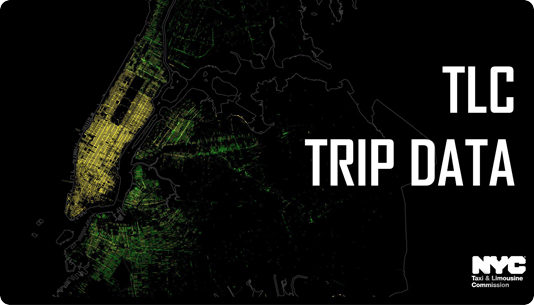
\includegraphics[width=0.9\textwidth]{images/nyc_taxi.png}
\caption[Taxi Dropoffs]{TLC Trip Record Data}
\end{figure}

The New York City Taxi and Limousine Commission (TLC) Trip Record Data \cite{nyc} consists of trip records from the yellow and green taxis.
Furthermore there are data from the For-Hire Vehicle (FHV).
The data includes information about capturing pick-up and drop-off locations, times, trip distances, fares, rate types, and driver-reported passenger counts.

To simplify the handling with the huge amount of data we used the scripts from the Github repository \cite{nyctaxigithub}, that is able to download all the data, provides the schema for PostgreSQL and consists of scripts to import the data.

\subsection{Specification}
To get a brief overview of the specification have a look at the following list.
\begin{itemize}[noitemsep, topsep=0pt]
\itemsep-0.5em
 \item[Format:]  CSV
 \item[Yellow:]  January 2009 - June 2017
 \item[Green:]  August 2013 - June 2017
 \item[FHV:]  January 2015 - June 2017
 \item[Taxi trips:] Over 1.1 billion \cite{billion}
 \item[Size:] 267 GB \cite{billion}
\end{itemize}

\subsection{Data subset}
Due to the fact that not all GPU databases are able to handle queries based on data larger than the GPU memory,
we had to shrink the dataset fitting into the available memory.

The GPU used on the server for the benchmark is a Nvidia Tesla K40m with 12 GB memory.
Hence we used the yellow and green taxi trip data of the year 2015, that has a size of 12 GB, too.
Consequently all queries fit into the GPU memory.


\newpage
\section{Queries}
\label{sec:queries}
The Queries were predefined by Prof. Stefan Keller and are inspired by the Google BigQuery examples \cite{bigquery}.
All the queries are listed below, the used syntax is able to run on MapD. \\


\begin{lstlisting}[language=sql, caption={Query 1, Counts all the yellow taxi trips},captionpos=b]
SELECT passenger_count, Avg(total_amount)
FROM   trips
GROUP  BY 1;
\end{lstlisting}


\begin{lstlisting}[language=sql, caption={Query 2, Calculates the average passenger amount per trip},captionpos=b]
SELECT cab_type_id, Count(*)
FROM   trips
GROUP  BY 1;
\end{lstlisting}

\begin{lstlisting}[language=sql, caption={Query 3, Sums the yearly amount of passengers},captionpos=b]
SELECT passenger_count, Extract(year FROM pickup_datetime), Count(*)
FROM   trips
GROUP  BY 1, 2;
\end{lstlisting}


\begin{lstlisting}[language=sql, caption={Query 4, Groups the amount of passenger by year regarding the trip distance},captionpos=b]
SELECT passenger_count, Extract(year FROM pickup_datetime), Cast(trip_distance AS INT), Count(*)
FROM   trips
GROUP  BY 1, 2, 3
ORDER  BY 2, 4 DESC;
\end{lstlisting}

\begin{lstlisting}[language=sql, caption={Query 5, Queries all trips in a certain bounding box},captionpos=b]
SELECT *
FROM   trips
WHERE  ( pickup_longitude BETWEEN -74.007511 AND -73.983479 )
       AND ( pickup_latitude BETWEEN 40.7105 AND 40.731071 ) LIMIT 10;
\end{lstlisting}


\begin{lstlisting}[language=sql, caption={Query 6, Determines the average speed of the yellow taxi trips by hour of the day in a bounding box},captionpos=b]
SELECT Extract(HOUR FROM pickup_datetime) AS h, AVG(trip_distance / NULLIF(TIMESTAMPDIFF(HOUR,pickup_datetime, dropoff_datetime),0)) AS speed
FROM   trips
WHERE  ( pickup_longitude BETWEEN -74.007511 AND -73.983479 )
       AND ( pickup_latitude BETWEEN 40.7105 AND 40.731071 )
       AND trip_distance > 0
       AND fare_amount / trip_distance BETWEEN 2 AND 10
       AND dropoff_datetime > pickup_datetime
       AND cab_type_id = 1
GROUP  BY h
ORDER  BY h;
\end{lstlisting}


\begin{lstlisting}[language=sql, caption={Query 7, Computes the average speed of the yellow taxi trips by hour of the day},captionpos=b]
SELECT Extract(HOUR FROM pickup_datetime) AS h, Avg(trip_distance / NULLIF(TIMESTAMPDIFF(HOUR, pickup_datetime, dropoff_datetime),0))AS speed
FROM   trips
WHERE  trip_distance > 0
       AND fare_amount / trip_distance BETWEEN 2 AND 10
       AND dropoff_datetime > pickup_datetime
       AND cab_type_id = 1
GROUP  BY h
ORDER  BY h;
\end{lstlisting}


\begin{lstlisting}[language=sql, caption={Query 8, Calculates the average speed of the yellow taxi trips by day of the week},captionpos=b]
SELECT Extract(DOW FROM pickup_datetime) AS dow, Avg(trip_distance / NULLIF(TIMESTAMPDIFF(HOUR,pickup_datetime,  dropoff_datetime), 0)) AS speed
FROM   trips
WHERE  trip_distance > 0
       AND fare_amount / trip_distance BETWEEN 2 AND 10
       AND dropoff_datetime > pickup_datetime
       AND cab_type_id = 1
GROUP  BY dow
ORDER  BY dow;
\end{lstlisting}


\begin{lstlisting}[language=sql, caption={Query 9, Determines the average speed of the yellow taxi trips by day of the week in a bounding box},captionpos=b]
SELECT Extract(DOW FROM pickup_datetime) AS dow, Avg(trip_distance / NULLIF(TIMESTAMPDIFF(HOUR,pickup_datetime,  dropoff_datetime), 0)) AS speed
FROM   trips
WHERE  ( pickup_longitude BETWEEN -74.007511 AND -73.983479 )
       AND ( pickup_latitude BETWEEN 40.7105 AND 40.731071 )
       AND trip_distance > 0
       AND fare_amount / trip_distance BETWEEN 2 AND 10
       AND dropoff_datetime > pickup_datetime
       AND cab_type_id = 1
GROUP  BY dow
ORDER  BY dow;
\end{lstlisting}

\newpage
\section{Results}
As already mentioned the queries of the benchmark were applied on a database without GPU acceleration,
in our case PostgreSQL 10.0 and a on MapD 3.3.1 a GPU powered database.
The dataset was introduced in section~\ref{sec:dataset} and the queries are listed in the section~\ref{sec:queries}.


\begin{minipage}{\textwidth}
  \begin{minipage}[b]{0.6\textwidth}
    \centering
     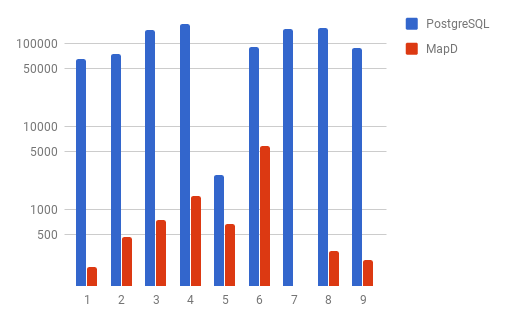
\includegraphics[width=1.0\textwidth,height=1.0\textheight,keepaspectratio]{images/cold_postgres_vs_mapd.png}
    \captionof{figure}{Diagram PostgreSQL vs. MapD cold}
    \label{fig:cold_postgres_vs_mapd}
  \end{minipage}
  \hfill
  \begin{minipage}[b]{0.4\textwidth}
    \centering
  \begin{tabular}{ |l|l|l| }
    \hline
    Query & PostgreSQL & MapD \\
    \hline
    1 & 64878 & 203 \\
    2 & 74404 & 456 \\
    3 & 145749 & 742 \\
    4 & 172592 & 1.431 \\
    5 & 2556 & 663 \\
    6 & 89029 & 5.756 \\
    7 & 150823 & 119 \\
    8 & 152883 & 315 \\
    9 & 87535 & 243 \\
    \hline
\end{tabular}
      \captionof{table}{Data PostgreSQL vs. MapD cold}
            \label{tab:cold_postgres_vs_mapd}
    \end{minipage}
 \end{minipage}


\begin{minipage}{\textwidth}
  \begin{minipage}[b]{0.6\textwidth}
    \centering
     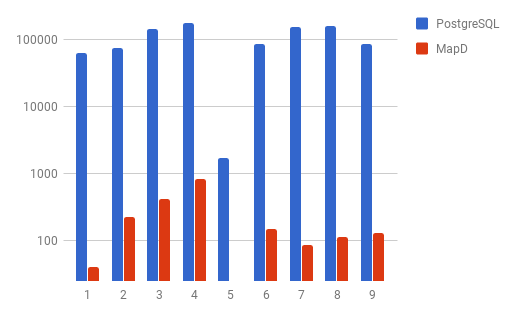
\includegraphics[width=1.0\textwidth,height=1.0\textheight,keepaspectratio]{images/warm_postgres_vs_mapd.png}
    \captionof{figure}{Diagram PostgreSQL vs. MapD warm}
    \label{fig:warm_postgres_vs_mapd}
  \end{minipage}
  \hfill
  \begin{minipage}[b]{0.4\textwidth}
    \centering
  \begin{tabular}{ |l|l|l| }
    \hline
    Query & PostgreSQL & MapD \\
    \hline
    1 & 62684 & 41 \\
    2 & 75140 & 223 \\
    3 & 142338 & 412 \\
    4 & 172052 & 840 \\
    5 & 1685 & 25 \\
    6 & 84439 & 149 \\
    7 & 150073 & 86 \\
    8 & 155107 & 115 \\
    9 & 86060 & 131 \\
    \hline
\end{tabular}
      \captionof{table}{Data PostgreSQL vs. MapD warm}
            \label{tab:warm_postgres_vs_mapd}
    \end{minipage}
 \end{minipage}



 \begin{minipage}{\textwidth}
  \begin{minipage}[b]{0.6\textwidth}
    \centering
     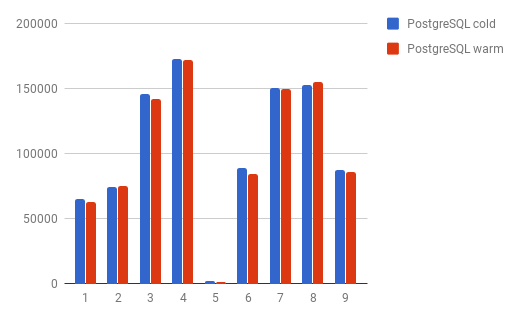
\includegraphics[width=1.0\textwidth,height=1.0\textheight,keepaspectratio]{images/postgres_cold_vs_warm.png}
    \captionof{figure}{Diagram PostgreSQL cold vs. PostgreSQL warm}
    \label{fig:postgres_cold_vs_warm}
  \end{minipage}
  \hfill
  \begin{minipage}[b]{0.4\textwidth}
    \centering
  \begin{tabular}{ |l|p{2cm}|p{2cm}| }
    \hline
    Query & PostgreSQL cold & PostgreSQL warm \\
    \hline
    1 & 64878 & 62684 \\
    2 & 74404 & 75140 \\
    3 & 145749 & 142338 \\
    4 & 172592 & 172052 \\
    5 & 2556 & 1685 \\
    6 & 89029 & 84439 \\
    7 & 150823 & 150073 \\
    8 & 152883 & 155107 \\
    9 & 87535 & 86060 \\
    \hline
\end{tabular}
      \captionof{table}{Data PostgreSQL cold vs. PostgreSQL warm}
            \label{tab:postgres_cold_vs_warm}
    \end{minipage}
 \end{minipage}



  \begin{minipage}{\textwidth}
  \begin{minipage}[b]{0.6\textwidth}
    \centering
     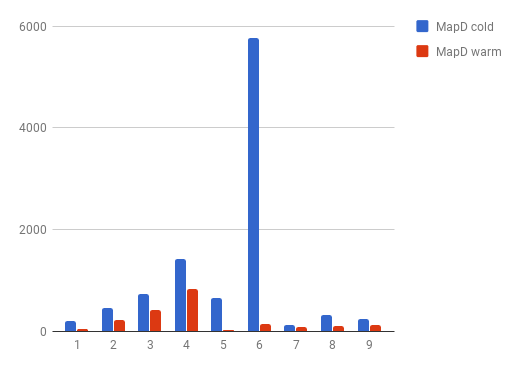
\includegraphics[width=1.0\textwidth,height=1.0\textheight,keepaspectratio]{images/mapd_cold_vs_warm.png}
    \captionof{figure}{Diagram MapD cold vs. MapD warm}
    \label{fig:mapd_cold_vs_warm}
  \end{minipage}
  \hfill
  \begin{minipage}[b]{0.4\textwidth}
    \centering
  \begin{tabular}{ |l|p{2cm}|p{2cm}| }
    \hline
    Query & MapD cold & MapD warm \\
    \hline
    1 & 203 & 41 \\
    2 & 456 & 223 \\
    3 & 742 & 412 \\
    4 & 1.431 & 840 \\
    5 & 663 & 25 \\
    6 & 5.756 & 149 \\
    7 & 119 & 86 \\
    8 & 315 & 115 \\
    9 & 243 & 131 \\
    \hline
\end{tabular}
      \captionof{table}{Data MapD cold vs. MapD warm}
            \label{tab:mapd_cold_vs_warm}
    \end{minipage}
 \end{minipage}


\appendix
\clearpage
\vspace*{\stretch{2.2}}
\begin{center}
\begin{minipage}{.25\textwidth}
\chapter*{Appendices}
\end{minipage}
\end{center}
\vspace{\stretch{3}}
\clearpage


\input{99_repositories}




\cleardoublepage

\phantomsection

\addcontentsline{toc}{chapter}{Bibliography}

\printbibliography

\end{document}
